%% LaTeX-Beamer template for KIT design
%% by Erik Burger, Christian Hammer
%% title picture by Klaus Krogmann
%%
%% version 2.1
%%
%% mostly compatible to KIT corporate design v2.0
%% http://intranet.kit.edu/gestaltungsrichtlinien.php
%%
%% Problems, bugs and comments to
%% burger@kit.edu

\documentclass[18pt]{beamer}
\usepackage[utf8x]{inputenc}
\usepackage{units}
\usepackage{booktabs}

%% CUSTOM
\usepackage{amsmath}
\usepackage{algpseudocode}

%% Definitions
\DeclareMathOperator{\div2}{div}
\renewcommand{\algorithmicrequire}{\textbf{Input:}}
\renewcommand{\algorithmicensure}{\textbf{Output:}}
\algnewcommand\algorithmicto{\textbf{to}}
\algrenewtext{For}[3]{\algorithmicfor\ $#1 \gets #2$ \algorithmicto\ $#3$ \algorithmicdo}
\algnewcommand\algorithmicod{\textbf{od}}
\algrenewtext{EndWhile}{\algorithmicod}
\algrenewtext{EndFor}{\algorithmicod}
%\AtBeginSection[]{%
%\begin{frame}<beamer> % do nothing in handouts
%    \frametitle{Überblick}
%    \tableofcontents[sectionstyle=show/shaded,
%    subsectionstyle=show/show/hide]
%\end{frame}
%}
%\AtBeginSubsection[]{%
%\begin{frame}<beamer> % do nothing in handouts
%    \frametitle{Überblick}
%    \tableofcontents[sectionstyle=show/shaded,
%    subsectionstyle=show/shaded/hide]
%\end{frame}
%}

%% SLIDE FORMAT

% use 'beamerthemekit' for standard 4:3 ratio
% for widescreen slides (16:9), use 'beamerthemekitwide'

\usepackage{templates/beamerthemekit}
%\usepackage{templates/beamerthemekitwide}

 %% TITLE PICTURE

 % if a custom picture is to be used on the title page, copy it into the 'logos'
 % directory, in the line below, replace 'mypicture' with the 
 % filename (without extension) and uncomment the following line
 % (picture proportions: 63 : 20 for standard, 169 : 40 for wide
 % *.eps format if you use latex+dvips+ps2pdf, 
 % *.jpg/*.png/*.pdf if you use pdflatex)


 \titleimage{banner}
 
 
%% Define some colors:
\definecolor{darkblue}{rgb}{0,0,.5}
\definecolor{darkgreen}{rgb}{0,.5,0}

 %% TITLE LOGO

 % for a custom logo on the front page, copy your file into the 'logos'
 % directory, insert the filename in the line below and uncomment it

\titlelogo{logo_150x150}
 
 % (*.eps format if you use latex+dvips+ps2pdf,
 % *.jpg/*.png/*.pdf if you use pdflatex)
 
 %% TikZ INTEGRATION
 
 % use these packages for PCM symbols and UML classes
 % \usepackage{templates/tikzkit}
 % \usepackage{templates/tikzuml}
 
 % the presentation starts here
 
\author{Dominik Muth - dominik.muth@student.kit.edu}
\institute{Institut f\"ur Informatik}


\title[Tutorium 6]{GBI Tutorium Nr. $2^5$}
\subtitle{Tutorium 6}
\date{28. November 2012}

% Bibliography



\begin{document}

	%title page
	\begin{frame}
		\titlepage
	\end{frame}

	%table of contents
	\begin{frame}{Outline/Gliederung}
		\tableofcontents
	\end{frame}
	
	
	
	\section{\"Ubungsblatt 5}
	\begin{frame} {Übungsblatt 5}
		\begin{block}{Aufgabe 5.1 b)}
			Ein Wort $w \in \{a,b\}^*$ ist genau dann in $L_b$, wenn das maximal lange Anfangsstück von w, das nur aus $a$a besteht, und das maximal lange Endstück von $w$, das nur aus $a$ besteht, gleiche Länge haben.
		\end{block}
	\end{frame}	
		
	
	
	
	\section{Wiederholung} 
	\begin{frame} {Wiederholung - Quiz}
		\begin{itemize}
			\item Schleifeninvarianten sind immer eindeutig. 
			\only<2-> {\color{red}$X$}\\
			\color{black}
					
			\item Aus einer Schleifeninvariante lässt sich der Sinn des Algorithmus herleiten.
			\only<3-> {\color{red}$X$}\\
			\color{black}
	
			\item $\neg (A \land B) \Leftrightarrow \neg A \lor \neg B$
			\only<4-> {\color{darkgreen}$\surd$}\\
			\color{black}
			
			\item $x^2$ ist eine surjektive Abbildung
			\only<5-> {\color{darkgreen}$\surd$\color{red}$X$}\\
			\color{black}
		\end{itemize}
	\end{frame}
	
	
	
	\begin{frame} {Wiederholung - Aufgaben}
		\begin{block}{Binäre Operationen}
			Geben Sie für folgende aussagenlogische Formeln jeweils einen 
			arithmetischen Ausdruck an, so dass das Ergebnis 
			den Wahrheitswerten der aussagenlogischen Formel entspricht. 
			Verwenden Sie für den Ausdruck nur die Operatoren +, - und 
			$\cdot$ sowie konstante Zahlen. 0 bzw. 1 repräsentiert dabei den
			 Wahrheitswert $falsch$ bzw. $wahr$.
			 
			 \begin{itemize}
			 	\item $ A \lor B$
			 	
			 	\item $ A \Rightarrow B $
			 	
			 	\item $ A \Leftrightarrow B $
			 \end{itemize}
		\end{block}
	\end{frame}
	
	
	
	\begin{frame} {Wiederholung}
		\begin{block}{Vollständige Induktion}
			Beweisen sie folgende Gleichung durch vollständige Induktion:\\
			\[ \sum_{i=1}^{n}(2i-1) = n^2 \]
		\end{block}
	\end{frame}
	
	
	
	\section{Zahlensysteme}
	\begin{frame}{Zahlensysteme}
		\begin{block}{Definition}
			Eine Zahl wird mit $Num_x$ zur Basis x dargestellt.\\
			
			\pause
			Beispiel: $Num_{10}$ ist definiert durch:\\
			
			
			\begin{align}
			Num_{10}(\epsilon) &=& 0 \\
			\forall v \in Z_{10}^*\forall w \in Z_{10} : Num_{10}(vw) 
			&=& 10 \cdot Num_{10}(v) + Num_{10}(w)
			\end{align}
			
		\end{block}
		
		\begin{Lemma}
			$Num_{10}$ ist durch Gleichung $1$ und $2$ wohldefiniert.\\
			\pause
			Wie beweisen wir das?
		\end{Lemma}
	\end{frame}
	
	
	\begin{frame}{Allgemein}
		\begin{block}{Für $Num_x$}
			\begin{align}
			Num_{x}(\epsilon) &=& 0 \\
			\forall v \in Z_{x}^*\forall w \in Z_{x} : Num_{10}(vw) 
			&=& x \cdot Num_{x}(v) + Num_{x}(w)
			\end{align}
		\end{block}
	\end{frame}
	
		
	
	\begin{frame}{Beispiel}
		\begin{block}{Beispiel für $Num_3$}
			$Num_3(12012)$\\
		\pause
			Nach Gleichung 2 $\Rightarrow Num_3(12012) = 3*Num_3(1201) + Num_3(2)$\\
		\pause
			$\Rightarrow^* 3*\bigg(3*\Big(3*\big(3*Num_3(1) )+Num_3(2)\big)+ Num_2(0)\Big)+Num_3(1)\bigg) + Num_3(2) $\\
		\pause
			\vspace{5pt}
			$= 81* Num_3(1) + 27* Num_3(2) + 9* Num_3(0) + 3* Num_3(1) + Num_3(2)$\\
		\pause
			\vspace{5pt}
			$ = 81* 1 + 27* 2 + 9 * 0 + 3 * 1 + 2$\\
		\pause
			\vspace{5pt}
			$ = 140$
		\end{block}
		
		\pause
		Kann man das ganze noch in einer anderen Form darstellen?
	\end{frame}
	
	
	\begin{frame}{Aufgaben}
		\begin{itemize}
			\item $\forall m \in \mathbb{N}_0 : Num_4({3}^m) = ?$\\
				\visible<2->{
					\color{darkgreen} 
					$4^m - 1$ 
					\color{black}}
					\pause
			\item Schreibe einen Algorithmus um die $Num_5(w)$ zu berechnen, 
			mit $w \in Z_5^*$. \\
			w(i) gibt das Zeichen an der i-ten Stelle zurück.
		\end{itemize}
	\end{frame}
	
	
	
	\section{Übersetzungen/Homomorphismen}
	\begin{frame}{Übersetzungen}
		\begin{block}{Warum?}
			\begin{itemize}
				\item Lesbarkeit (z.B. Deutsch statt Chinesisch)
				
				\pause
				\item Kompression (z.B. Zip-Dateien)
				
				\pause
				\item Verschlüsselung (z.B. https)
				
				\pause
				\item Fehlererkennung und Korrektur 
			\end{itemize}
		\end{block}
	\end{frame}
	
	
	\begin{frame}{Homomorphismen}
		\begin{block}{Was ist das?}
			Ein Homomorphismus hat die Eigenschaft, 
			dass er strukturerhaltend ist, 
			das bedeutet z.B. für Abbildungen auf den natürlichen Zahlen:\\
			\vspace{10pt}
			$\forall x,y \in \mathbb{N}_0 : f(x) + f(y) = f(x+y)$ 
		\end{block}
		
		\pause
		
		\begin{exampleblock}{Beispiel}
			$f(x) = 2x$
		\end{exampleblock}
	\end{frame}
	
	
	\begin{frame}{Homomorphismen}
		\begin{block}{Wie auf Wörter übertragen?}
			Eigenschaften, welche sich ausnutzen lassen:\\
			\begin{itemize}
				\item Wörter lassen sich konkatenieren
				
				\item Wörter, lassen sich auf Werte abbilden
			\end{itemize}
		\end{block}
		
		\pause		
		
		\begin{exampleblock}{Beispiel}
			-- $h(a) = 001$ und $h(b) = 1101$\\
			-- dann ist $h(bba) = h(b)h(b)h(a) = 1101 \cdot 1101 \cdot 001 = 11011101001$\\
			\vspace{10pt}
			\visible<3->{Warum?}
		\end{exampleblock}
	\end{frame}
	
	
	\begin{frame}{Homomorphismen}
		\begin{block}{Was gibt es allgemein zu beachten?}
			\begin{itemize}
				\item $\epsilon$-freier Homomorphismus: \pause Warum?
				
				\pause
				\item $\forall x,y,z \in A : x \cdot y \not= z \Rightarrow h(x) \cdot h(y) \not= h(z)$
				
				\pause
				\item präfixfreier Code: für keine zwei verschiedenen Symbole 
				$x1, x2 \in A$ gilt: $h(x1)$ ist ein Präfix von $h(x2)$.
			\end{itemize}
		\end{block}
		
		\vspace{15pt}
		\visible<5->{Gibt es Ausnahmen?}
	\end{frame}
	
	
	\begin{frame}{Aufgaben}
		\begin{block}{}
			Gegeben sei $A = \{a,b,c\}$ mit:\\
			$h(a) = 1011$, $h(b) = 0110$, $h(c) = 111 $
			\begin{itemize}
				\item ist h präfixfrei?\\
					\visible<2->{\color{darkgreen} ja \color{black}}
					
				\item Berechnen Sie $h(aacbabca)$\\
					\visible<3->{\color{darkgreen}
					 101110111110110101101101111011 \color{black}}
					 
				\item Berechnen sie $w$ für welches gilt: 
				$h(w) = 01101111111011111011011110110110$\\
				\visible<4->{\color{darkgreen} bccacbcab \color{black}}
			\end{itemize}
		\end{block}
	\end{frame}
	
	
	\section{Huffman-Codierung}
	\begin{frame}{Huffman-Codierung}
		\begin{block}{Allgemein Vorgehensweise}
			\begin{itemize}
				\item Tabelle aufstellen, wie oft kommt jedes Element vor?
				
				\pause
				\item Baum aufstellen, Blätter sind die Elemente.
				
				\pause
				\item Elemente mit niedrigster Häufigkeit zu neuem Knoten
				 zusammenführen und addierte Häufigkeit in Knoten schreiben.
				 
				\pause
				\item solange Wiederholen bis nur noch die Wurzel übrig ist.
				
				\pause
				\item Kanten beschriften, Kanten nach links mit 1 und Kanten nach rechts mit 0, oder anders herum.
					
			\end{itemize}
		\end{block}
	\end{frame}
		
	\begin{frame}{Huffman-Codierung}
		\begin{exampleblock}{Beispiel}
			\begin{itemize}
			\item Kodierung für "w = badcfehg"
			
			\pause
			\item Kodierung für ein Wort, in welchem a einmal, b zweimal, c 4-mal, d 8-mal, e 16-mal, f 32-mal, g 64-mal und h 128-mal vorkommt
			\end{itemize}
		\end{exampleblock}
	\end{frame}	
	
	
	\begin{frame}{Huffman-Codierung}
		Wie sieht es mit der Codierung von $w = aaaaaabbbbbcccc$ aus?\\
		\vspace{15pt}
		
		\visible<2-> {
			Lässt sich das ganze noch optimieren?
		}
	\end{frame}		
	
	
	\section{Aufgaben}
	\begin{frame}
		\begin{block}{}
			Kodiere folgende Wörter mit der Huffman-Codierung:
			\begin{itemize}
				\item abcbcaaa
				\item ababababab
				\item hello$\textvisiblespace$world
			\end{itemize}
		\end{block}	
	\end{frame}
	
	
	
	
	\section{Fragen}
	\begin{frame} {Fragen}
		\begin{itemize}
			\item Fragen zum Stoff?
			\item Fragen zum n\"achsten \"Ubungsblatt?
			\item Generelle Fragen?
			\item Feedback?
		\end{itemize}
	\end{frame}

		
	\begin{frame} {EOF}
		\begin{center}
			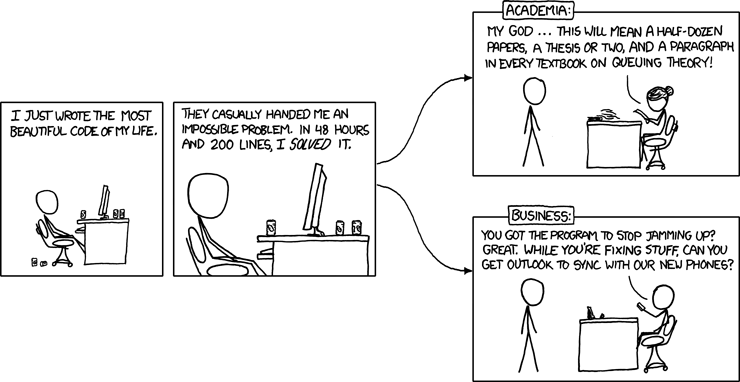
\includegraphics[scale=0.45]{graphics/eof6.png}\\
			\tiny $source: http://imgs.xkcd.com/comics/academia\_vs\_business.png$
		\end{center}
	\end{frame}

\end{document}
